
\section{The \pkg{sbtools} package}

With \pkg{sbtools}, our goal was to allow complete
access to the ScienceBase web service API in a flexible, lightweight,
R package. The package imports a minimal number of external packages
to support core functionality. More advanced data access (e.g., Geospatial
web services) are supported through suggested packages to keep the basic
install lightweight and simple on all platforms. Within R, \pkg{sbtools}
is designed to keep most interactions simple and includes internal
handling of complex web service interactions (e.g., authentication) to
simplify use for end-users.

Below, we describe briefly the core functions available in \pkg{sbtools}
and discuss the unique features of ScienceBase that \pkg{sbtools}
exposes to R users.


\subsection{Data access API}
The data access functionality of \pkg{sbtools} makes it easy to
access any public item's data, attached files and metadata. All items
in ScienceBase have a unique identifier that can be used to directly
access specific items.

\begin{example}
> test_item = item_get("4f4e4b24e4b07f02db6aea14")
> test_item
<ScienceBase Item>
  Title: Coastal-change and glaciological maps of Antarctica
  Creator/LastUpdatedBy:      /
  Provenance (Created / Updated):  2010-10-06T04:25:43Z / 2014-07-21T17:45:42Z
  Children: FALSE
  Item ID: 4f4e4b24e4b07f02db6aea14
  Parent ID: 4f4e4771e4b07f02db47e1e4
\end{example}

For convenience, \pkg{sbtools} defines an \code{sbitem} object, which is
returned by \pkg{sbtools} functions when referencing objects. The underlying
data structure is a list. All available metadata for an item can be listed
and accessed in the same way as a named list.

\begin{example}
> names(test_item)
 [1] "link"              "relatedItems"      "id"
 [4] "identifiers"       "title"             "citation"
 [7] "provenance"        "hasChildren"       "parentId"
[10] "contacts"          "webLinks"          "browseCategories"
[13] "browseTypes"       "tags"              "dates"
[16] "facets"            "files"             "distributionLinks"
[19] "previewImage"

> item_get(test_item)$citation
[1] "Geological Survey (U.S.), 1999-08-05, Coastal-change
and glaciological maps of Antarctica:  Fact SheetCoastal-change and
glaciological maps of Antarctica."
\end{example}

On ScienceBase, all items are organized in a tree structure, with one
parent and potentially many children. \pkg{sbtools} allows the user to
easily traverse the tree structure. For example, in some projects, the hierarchy has
important meaning. For other projects, it may relates to the user or
organizational owner of the data.

\begin{example}
#parent ID always available as item attribute
> parent = item_get(test_item$parentId)
> parent
  Title: USGS Publications Warehouse
  Creator/LastUpdatedBy:      /
  Provenance (Created / Updated):  2012-02-29T15:42:41Z / 2014-07-08T21:42:20Z
  Children: TRUE
  Item ID: 4f4e4771e4b07f02db47e1e4
  Parent ID: 4f4e4771e4b07f02db47e1da

#getting sibling items
> item_list_children(parent)
[1] "55b98fbee4b08f6647be5179" "541d45a4e4b0f68901ec30ef"
[3] "55b361b3e4b09a3b01b5daad" "53516ef9e4b05569d8059f34"
[5] "4f4e4ab2e4b07f02db66f5e3" "5351704ee4b05569d805a2e4"
\end{example}

ScienceBase items may have data or metadata files attached to them.
You can list and download attached files directly using \pkg{sbtools}.

\begin{example}
#returns files attached to item
item_list_files(test_item)
#returns local path to downloaded files
item_file_download(test_item, dest_dir = tempdir())
\end{example}

ScienceBase has special functionality when certain data types are
stored. One example is spatial data. When spatial data are properly
tagged and uploaded to ScienceBase, they can be accessed using OGC
web services. \pkg{sbtools} has included ability to access the Web
Feature Service (WFS) available for certain items.

\begin{example}
#Source non-sbtools-required but useful mapping packages
library(maps)
library(sp)
#an item with an included OGC WFS service
layer = item_get_wfs('55e372b9e4b05561fa208212')
map('state', regions='iowa')
plot(layer, add=TRUE)
\end{example}

%this figure code is demo\figure_map_code.R
% feel free to improve
 \begin{figure}[htbp]
   \centering
   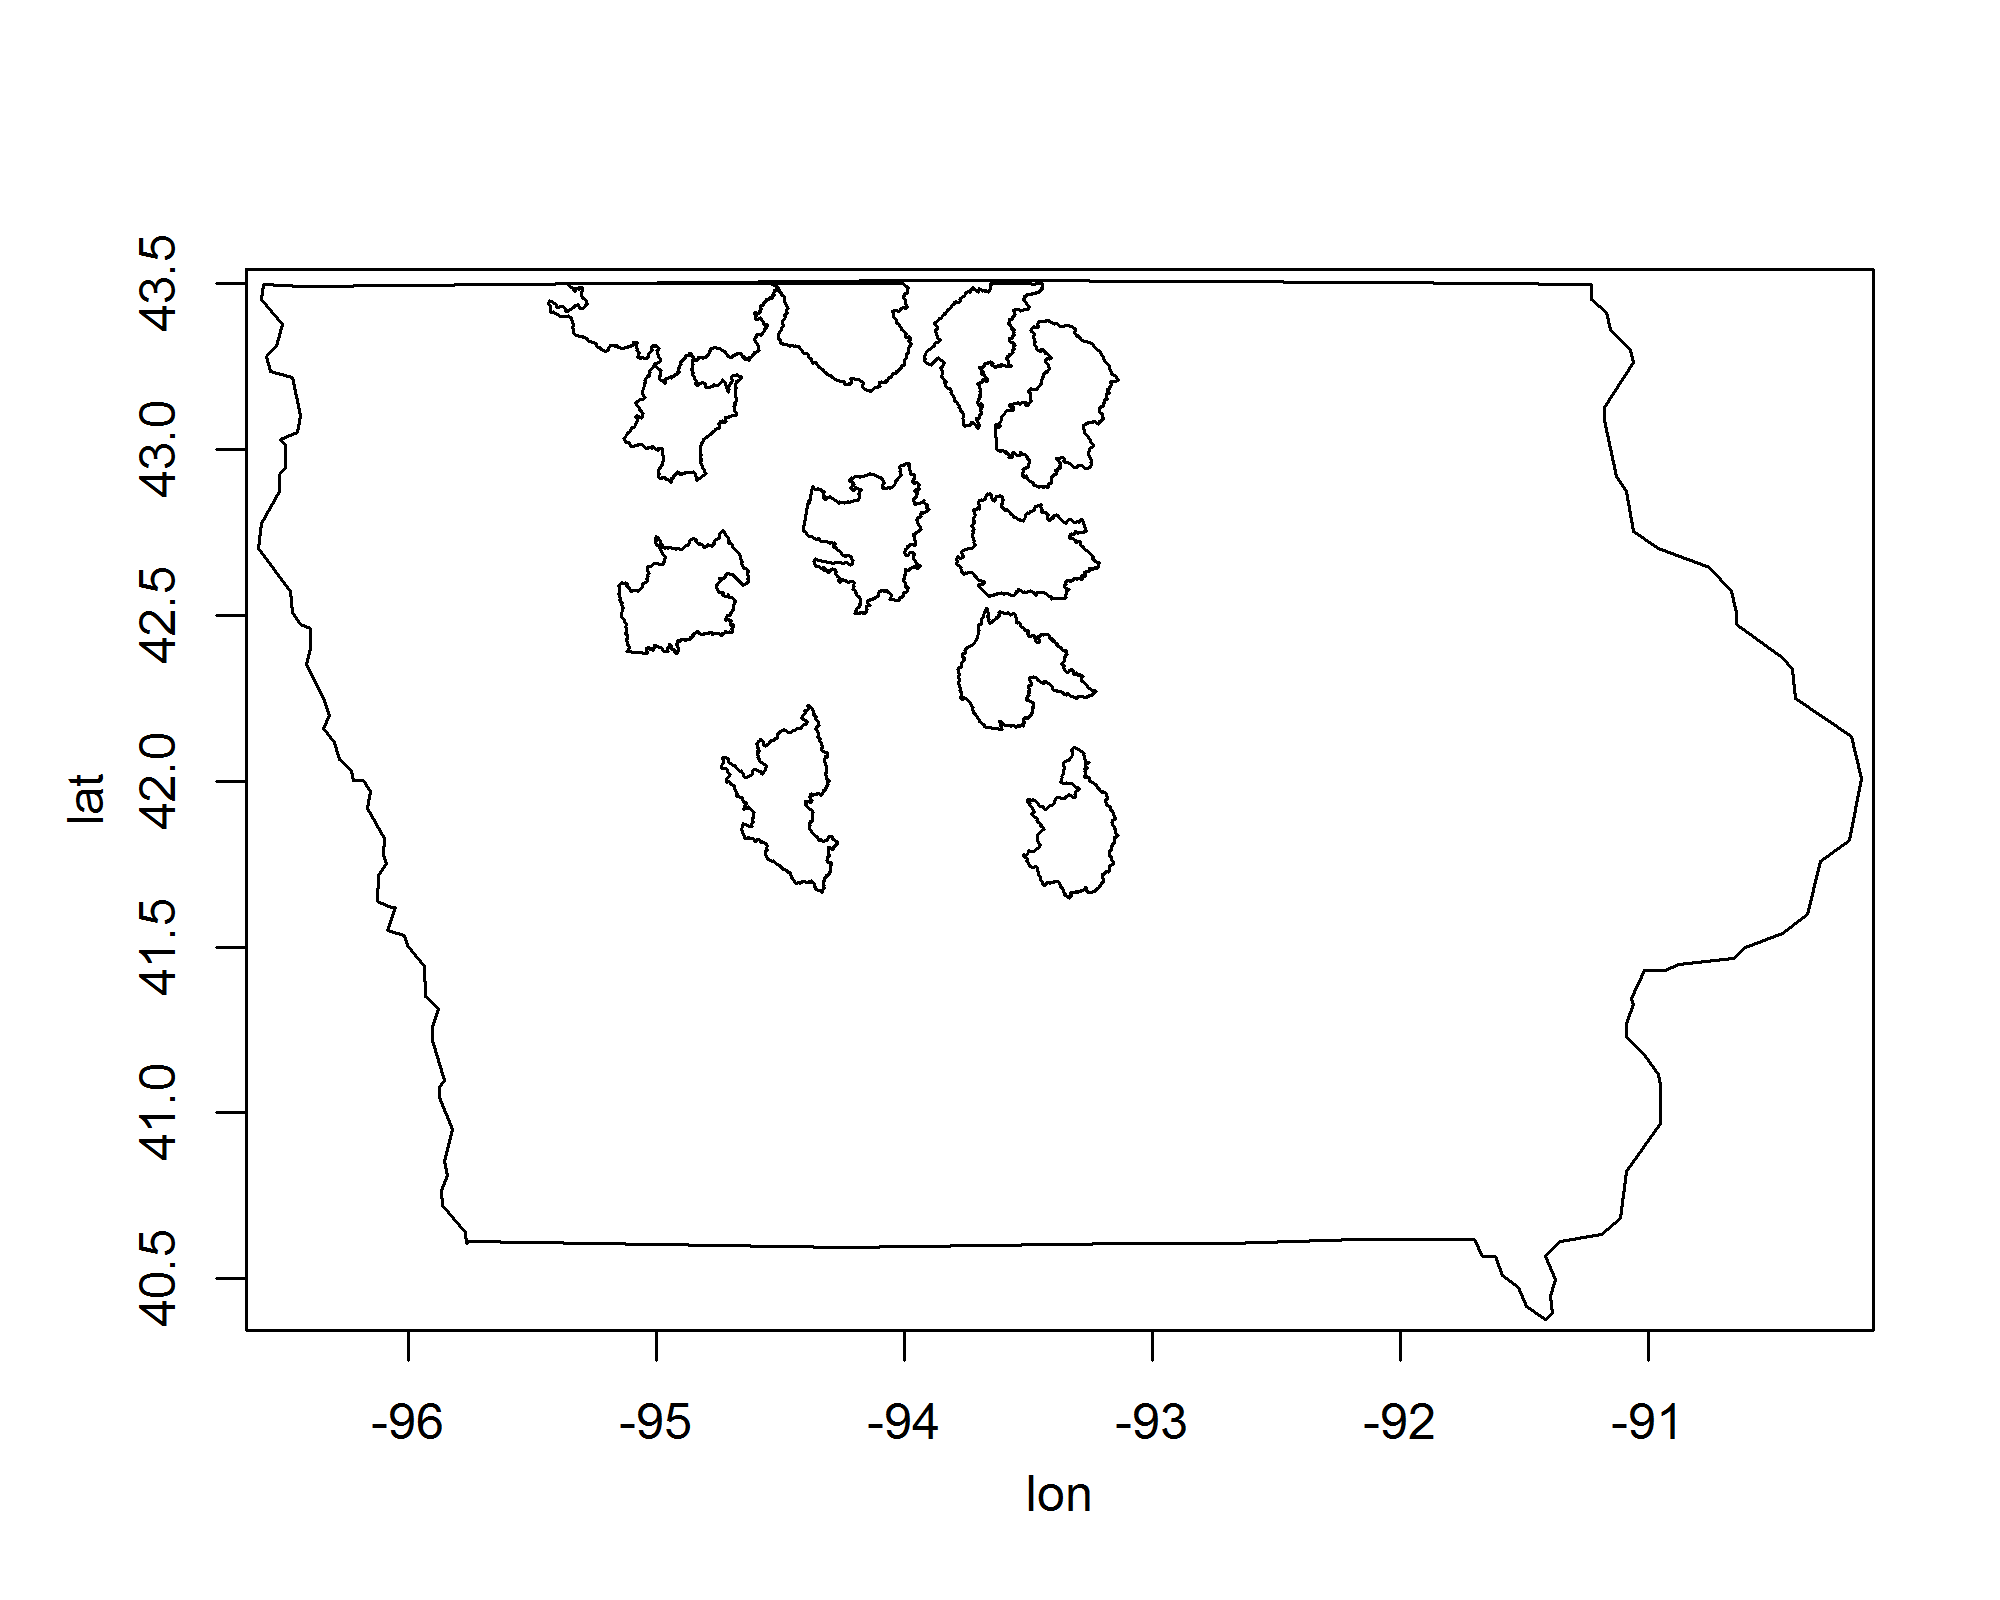
\includegraphics{mapfig}
   \caption{An example spatial dataset from ScienceBase,
   visualized on top of the outline for the state of Iowa}
   \label{figure:iowafig}
 \end{figure}


\subsection{Search API}
To support advanced and powerful data discovery, all data
in ScienceBase is indexed and made available through a flexible
search interface. \pkg{sbtools} offers several query
functions with different levels of search detail, from
basic, text-only to advanced, and low-level metadata specific search
functionality.


Convenient query wrappers are included to support the most common
query types. These include queries based on free text, date-time range,
geospatial bounding box, Digial Object Identifier (DOI) and data types.
Below are introductory examples. For presentaiton, we use the \code{limit}
parameter to limit all queries to the first 2 results. Further details
for each query type are available in the package documentation.

ScienceBase items have a number of different metadata fields that contain
date-time information. For example, items can have attached date-time
data which may include creation, modification, report, collection, or
publication date. To support the many different options, \code{query\_sb\_date()}
includes the \code{date\_type} parameter. Different parameter options can then
yield different results.

\begin{example}
#Query recently updated
> query_sb_date(Sys.time(), Sys.time(), date_type='lastUpdated', limit=2)
[[1]]
<ScienceBase Item>
  Title: US Topo
  Creator/LastUpdatedBy:      /
  Provenance (Created / Updated):  2012-03-05T22:46:14Z / 2016-02-01T12:11:58Z
  Children: TRUE
  Item ID: 4f554236e4b018de15819c85
  Parent ID: 4f552e93e4b018de15819c51

[[2]]
<ScienceBase Item>
  Title: USGS US Topo 7.5-minute map for Boyer, IA 2013
  Creator/LastUpdatedBy:      /
  Provenance (Created / Updated):  2014-05-01T08:13:22Z / 2016-02-01T10:21:18Z
  Children: FALSE
  Item ID: 53620222e4b0c409c627ec57
  Parent ID: 5061bc99e4b0ce47085a8d03

#query for data published in the 1970's
> query_sb_date(as.POSIXct('1970-01-01'), as.POSIXct('1980-01-01'), date_type='Publication', limit=2)
[[1]]
<ScienceBase Item>
  Title: Common marsh plants of the United States and Canada
  Creator/LastUpdatedBy:      /
  Provenance (Created / Updated):  2010-10-22T22:24:18Z / 2014-07-05T04:55:27Z
  Children: FALSE
  Item ID: 4f4e4b24e4b07f02db6ae651
  Parent ID: 4f4e4771e4b07f02db47e1e4

[[2]]
<ScienceBase Item>
  Title: Structure and mineralization of Precambrian rocks in the Galena-Roubaix district, Black Hills, South Dakota
  Creator/LastUpdatedBy:      /
  Provenance (Created / Updated):  2010-10-23T00:28:32Z / 2014-07-21T20:14:53Z
  Children: FALSE
  Item ID: 4f4e4b14e4b07f02db6a47a6
  Parent ID: 4f4e4771e4b07f02db47e1e4

\end{example}

Each item can be described by a data type tag. Because this field is free-text, it can take on a
number of different values. The function \code{sb\_datatypes()} returns the list of currently used
data type tags on ScienceBase. \code{query\_sb\_datatype} can be used to query for items described
with a specific data type.

\begin{example}
#List first 50 available data types
> sb_datatypes(limit = 50)
 [1] "Application"                                 "ArcGIS Map Package"                "ArcGIS REST Map Service"
 [4] "ArcGIS Service Definition"                   "ArcIMS Catalog"                    "ArcIMS Metadata"
 [7] "BASIS+ Project"                              "BASIS+ Subtask"                    "BASIS+ Task"
[10] "Book Citation"                               "Citation"                          "Clearinghouse"
[13] "Collection"                                  "Conference Citation"               "Digital Map - Beta"
[16] "Document"                                    "Downloadable"                      "Electronic Book Citation"
[19] "GeoProcessing Service"                       "GeoTIFF"                           "Glass Plate Photonegative"
[22] "High-Resolution Scanned Topo Maps"           "Journal Citation"                  "Live Data"
[25] "Low-Resolution Scanned Topo Maps PDF"        "Map Service"                       "National Map Digital Map - Beta"
[28] "NetCDF OPeNDAP Service"                      "News"                              "NGTOC Open File Report GeoPDF"
[31] "NSDI Cooperative Agreements Program Project" "Offline Data"                      "OGC WFS Layer"
[34] "OGC WMS Layer"                               "OGC WMS Service"                   "Photonegative"
[37] "Print"                                       "Raster"                            "Report"
[40] "Report Citation"                             "ScienceBase Citation"              "ScienceBase Information Article"
[43] "ScienceBase Project"                         "sdc"                               "Shapefile"
[46] "Static Map Image"                            "Thesis Citation"                   "US Topo"

#Query ScienceBase for US Topographic data
> query_sb_datatype('US Topo')
[[1]]
<ScienceBase Item>
  Title: USGS Geoscience Data Catalog
  Creator/LastUpdatedBy:      /
  Provenance (Created / Updated):  2014-05-22T19:06:52Z / 2015-02-05T18:41:43Z
  Children: TRUE
  Item ID: 537e4acce4b05ed6215c0a18
  Parent ID: 527cf4ede4b0850ea05182ee

[[2]]
<ScienceBase Item>
  Title: TNC repeat photographs
  Creator/LastUpdatedBy:      /
  Provenance (Created / Updated):  2014-10-16T22:11:20Z / 2015-04-01T22:25:37Z
  Children: TRUE
  Item ID: 54404288e4b0b0a643c73143
  Parent ID: 54247f49e4b037b608f9edd1
\end{example}


On ScienceBase, the preferred way of storing an item's DOI is using the custom item
identifier fields. \code{query\_sb\_doi()} can query those fields specifically for
a DOI. Here are examples of querying items by DOI on ScienceBase.
\begin{example}
#some item DOI's have 'doi:' appended to the front of them for some reason
query_sb_doi('doi:10.5066/F7M043G7')
[[1]]
<ScienceBase Item>
  Title: 2013 Raw Ground Penetrating Radar Data on Alaska's Glaciers
  Creator/LastUpdatedBy:      /
  Provenance (Created / Updated):  2015-06-15T16:55:03Z / 2015-12-15T20:39:06Z
  Children: TRUE
  Item ID: 557f0367e4b023124e8ef621
  Parent ID: 5474ec49e4b04d7459a7eab2

#others do not
query_sb_doi('10.1126/science.aab1345')
[[1]]
<ScienceBase Item>
  Title: High-rate injection is associated with the increase in U.S. mid-continent seismicity
  Creator/LastUpdatedBy:      /
  Provenance (Created / Updated):  2015-06-23T19:52:11Z / 2015-07-06T21:08:26Z
  Children: FALSE
  Item ID: 5589b8ebe4b0b6d21dd63b5a
  Parent ID: 511033e1e4b048b5cead8548
\end{example}

Data with a geospatial component to their data or metadata can be queried using a
Lat/Lon bounding box. \pkg{sbtools} provides the function \code{query\_sb\_spatial()}
which can be used by directly supplying lat/long bounding box coordinates, or has
helpful parameters that can use the bounding box from \code{sp} spatial objects. Because
spatial functionality requires packages beyond those imported by \pkg{sbtools} by default,
these functions will require the \pkg{sp} and \pkg{gdalUtils} packages be installed.

\begin{example}
##specify the lat/long corners of the bounding box
> query_sb_spatial(bb_min=c(-104.4, 37.5), bb_max=c(-95.1, 41.0))
[[1]]
<ScienceBase Item>
  Title: National Fish Habitat Partnership Data System
  Creator/LastUpdatedBy:      /
  Provenance (Created / Updated):  2012-02-29T15:42:43Z / 2015-11-12T20:19:30Z
  Children: TRUE
  Item ID: 4f4e4773e4b07f02db47e241
  Parent ID: 4f4e4760e4b07f02db47df9c

[[2]]
<ScienceBase Item>
  Title: Geo Data Portal Catalog
  Creator/LastUpdatedBy:      /
  Provenance (Created / Updated):  2015-02-12T22:03:18Z / 2015-11-24T22:38:06Z
  Children: TRUE
  Item ID: 54dd2326e4b08de9379b2fb1
  Parent ID: 4f4e4760e4b07f02db47df9c

##You can also use the bounding box of an sp spatial data object
#grab an sp object from a pre-determined ScienceBase Item
> layer = item_get_wfs('55e372b9e4b05561fa208212')

#get items in that BB
> query_sb_spatial(layer, limit=2)
[[1]]
<ScienceBase Item>
  Title: National Fish Habitat Partnership Data System
  Creator/LastUpdatedBy:      /
  Provenance (Created / Updated):  2012-02-29T15:42:43Z / 2015-11-12T20:19:30Z
  Children: TRUE
  Item ID: 4f4e4773e4b07f02db47e241
  Parent ID: 4f4e4760e4b07f02db47df9c

[[2]]
<ScienceBase Item>
  Title: USGS Denver Library Photographic Collection
  Creator/LastUpdatedBy:      /
  Provenance (Created / Updated):  2013-05-21T16:28:19Z / 2016-01-04T15:44:20Z
  Children: TRUE
  Item ID: 519ba0a3e4b0e4e151ef5dd9
  Parent ID: 4f4e4771e4b07f02db47e1da

\end{example}

Lastly, \pkg{sbtools} offers advanced access to all query capabilities through
the \code{query\_items()} and \code{query\_sb()} functions. \code{query\_items()} allows
the user to supply a list of query parameters (options described in the documentation),
submit that query to ScienceBase, and receive the raw HTTP response (as an \pkg{httr}
response object). \code{query\_sb()} provides a convenient wrapper that parses the output
into a list of \code{sbitem} objects and also does proper result paging when the requested
return length (limit) is over 1000 items. All advanced search options can be experimented
with via the  \href{https://www.sciencebase.gov/catalog/items/queryForm}
{online advanced search interface}.

\begin{example}

# query_sb can be used for combined search criteria
> query_sb(list(q = "water", folderId = '504216b9e4b04b508bfd337d', broserCategory = 'Image'), limit=2)
[[1]]
<ScienceBase Item>
  Title: Encyclopedia of Water Science
  Creator/LastUpdatedBy:      /
  Provenance (Created / Updated):  2013-04-18T15:06:38Z / 2013-04-18T15:06:38Z
  Children: FALSE
  Item ID: 51700bfee4b05024ef3cd4ef
  Parent ID: 504216b9e4b04b508bfd337d

[[2]]
<ScienceBase Item>
  Title: Introduction to special section on Impacts of Land Use Change on Water Resources
  Creator/LastUpdatedBy:      /
  Provenance (Created / Updated):  2013-04-18T15:07:35Z / 2013-04-18T15:07:35Z
  Children: FALSE
  Item ID: 51700c37e4b05024ef3cd4fd
  Parent ID: 504216b9e4b04b508bfd337d

\end{example}


\subsection{ScienceBase authentication}
In addition to the large collection of open, reusable datasets and
useful metadata ScienceBase has to offer, it is
also a platform for sharing and collaboration on private, in-progress
data available only through authenticated access. To enable
private data contribution and access,
\pkg{sbtools} has built-in support for persistent
authentication of R sessions.

Authentication in \pkg{sbtools} is handled through the persistence of
an authenticated session. By storing only the session, we do not need to
store the plaintext password, which could represent a security issue. This
session state is persisted between function calls by the package. While
expiration of the session can be difficult to predict, \pkg{sbtools}
makes a best effort to supply the user with meaningful error messages.

The authentication function \code{authenticate\_sb()} can accept a username
and password. Alternatively, to prevent plaintext passwords in R history,
the password can be omitted and will be requested by R interactively.
Authentication is persisted by the package, allowing for a single sign-in
and no tracking of usernames, passwords, or sessions during interactive or
script-based use.

%Authentication in sbtools
\begin{example}
#to start an authenticated session
> authenticate_sb('username@usgs.gov')
> is_logged_in()
[1] TRUE
> session_logout()
> is_logged_in()
[1] FALSE
\end{example}

Most functions in \pkg{sbtools} can be used both anonymously and when
authenticated. This includes all query and data retrieval functions.
When authenticated, these functions may return different results or fail
depending on the specific task. For example, when trying to access
a private item using \code{item\_get()}, you must be authenticated, otherwise
it will throw and error ScienceBase does not differentiate between a missing
item and an item you don't have permission to access. Search follows a similar
pattern. When querying items with \code{query\_sb()}, public items are always
visible while private items are not visible unless authenticated.

\begin{example}
#Attempt to get a private item
> item_get('55de0027e4b0518e354dfcf0')
 Error: Item not found for ID=55de0027e4b0518e354dfcf0. Either the
 item does not exist or the item is secured and requires authentication to access.

#Get private item while authenticated
> authenticate_sb('username@usgs.gov')
> item_get('55de0027e4b0518e354dfcf0')
 <ScienceBase Item>
  Title: Example Private Item
  Creator/LastUpdatedBy:     username@usgs.gov / username@usgs.gov
  Provenance (Created / Updated):  2015-08-26T18:06:31Z / 2015-12-30T14:59:27Z
  Children: FALSE
  Item ID: 55de0027e4b0518e354dfcf0
  Parent ID: 54257d8fe4b0e641df8b50af

#search expands to include user's private items when authenticated
#query while authenticated
> query_sb(list(q='username@usgs.gov'))
 <ScienceBase Item>
  Title: Example Private Item
  Creator/LastUpdatedBy:     username@usgs.gov / username@usgs.gov
  Provenance (Created / Updated):  2015-08-26T18:06:31Z / 2015-12-30T14:59:27Z
  Children: FALSE
  Item ID: 55de0027e4b0518e354dfcf0
  Parent ID: 54257d8fe4b0e641df8b50af

> session_logout()
> query_sb(list(q='username@usgs.gov'))
list()
\end{example}

%Examples of authentication and other auth-related functions (check and such)

\subsection{Data editing and upload API}
For authenticated users, \pkg{sbtools} has functionality to support
the full data lifecycle. This includes the creation, editing and removal
of items. Because item editing and creation cannot be done anonymously,
this functionality only works while authenticated.

When we create new items, the only required inputs are "Parent Item" and "title". All
items must have a non-empty title and a parent item. ScienceBase makes basic item creation
easy as all users have a personal home folder (called "My Items" on ScienceBase) and by default,
new items are created with that parent. The funciton \code{user\_id()} retrieves the
unique identifier for the user's home folder.

\begin{example}
#create new item, by default under "My Items" parent
> new_item = item_create(title='new test item')
> new_item
<ScienceBase Item>
  Title: new test item
  Creator/LastUpdatedBy:     username@usgs.gov / username@usgs.gov
  Provenance (Created / Updated):  2016-01-27T19:48:28Z / 2016-01-27T19:48:28Z
  Children: FALSE
  Item ID: 56a91f0ce4b0b28f1184dda8
  Parent ID: 54257d8fe4b0e641df8b50af
\end{example}

Once an item is created, we can edit the metadata or attach data files to that
item using \pkg{sbtools}.

\begin{example}
#giving the item a new title
> edited_item = item_update(new_item, list(title='new updated item'))
> edited_item
<ScienceBase Item>
  Title: new updated item
  Creator/LastUpdatedBy:     lwinslow@usgs.gov / lwinslow@usgs.gov
  Provenance (Created / Updated):  2016-01-27T19:48:28Z / 2016-01-27T19:50:21Z
  Children: FALSE
  Item ID: 56a91f0ce4b0b28f1184dda8
  Parent ID: 54257d8fe4b0e641df8b50af

#appending files to item
> item_list_files(new_item)
data frame with 0 columns and 0 rows

> item_append_files(edited_item, 'test.dat')
> item_list_files(edited_item)
      fname size     url
1 README.md 1282     https://www.sciencebase.gov/[long URL truncated]


\end{example}

A full set of functions is also provided to modify and delete attached
files and delete items.

\begin{example}
#files can be selectively replaced with files of the same name
> item_list_files(edited_item)
      fname size     url
1 README.md 1282     https://www.sciencebase.gov/[long URL truncated]

# all=FALSE replaces files one by one, otherwise all files are removed
# before uploading the new files
> item_replace_files(new_item, 'README.md', all = FALSE)
> item_list_files(edited_item)
      fname size     url
1 README.md 608     https://www.sciencebase.gov/[long URL truncated]

#our item is easily deleted as well (use with caution, there is no confirmation)
> item_rm(edited_item)

> item_get(edited_item)
Error: Item not found for ID=56a91f0ce4b0b28f1184dda8. Either the item does
not exist or the item is secured and requires authentication to access.
\end{example}


\subsection{SB Item identifiers}
One advanced and useful feature ScienceBase has is the ability to assign any
number of custom item identifiers to items. The custom identifiers are made up
of three parts: Scheme, Type and Key. Combined, these create a unique identifier.
There are some standard Schemes used in ScienceBase. For example, DOIs (Digital
Object Identifier) are stored as item identifiers with the scheme
"https://www.sciencebase.gov/vocab/category/item/identifier" and type "DOI".

\pkg{sbtools} can edit and query custom item identifiers using two functions:
\code{item\_update\_identifier} and \code{query\_item\_identifier}.

\begin{example}
#create two items and assign custom identifiers
> ident_item = item_create(title='test data')
> item_update_identifier(ident_item, scheme='proj2', type='data', key='dataset1')
> ident_item = item_create(title='test publication')
> item_update_identifier(ident_item, scheme='proj2', type='publication', key='pdf1')

#query for created item
> query_item_identifier(scheme='proj2', type='publication', key='pdf1')
             title                       id
1 test publication 56a9371ee4b012c193aa3d65

\end{example}

The three-part identifier can be especially useful as a way to organize and
access project data. All three parts can be quieried to access specific items
directly. But the hierarchical nature can be used to query groups of items as well.
For example, all items within the same project could be created with the same
scheme. More specifically, a project might have multiple types of items, giving
users the ability to query items based on the project and category.

\begin{example}
#query all items in 'proj2'
> query_item_identifier(scheme='proj2')
             title                       id
1 test publication 56a9371ee4b012c193aa3d65
2        test data 56a93777e4b012c193aa3d68

#query just data items for a project
> query_item_identifier(scheme='proj2', type='data')
      title                       id
1 test data 56a93777e4b012c193aa3d68

\end{example}


